\documentclass{scrartcl}
\usepackage[utf8]{inputenc} 
\usepackage[T1]{fontenc}
\usepackage{lmodern}
\usepackage[ngerman]{babel}
\usepackage{courier}
\usepackage{amsmath}
\usepackage{graphicx}
\usepackage{multicol}
\usepackage{geometry}
\usepackage{authblk}
\usepackage[font=scriptsize, labelfont=bf]{caption}
\usepackage{listings}
\usepackage{color}
\newenvironment{Figure}
  {\par\medskip\noindent\minipage{\linewidth}}
  {\endminipage\par\medskip}
  
\definecolor{dkgreen}{rgb}{0,0.6,0}
\definecolor{gray}{rgb}{0.5,0.5,0.5}
\definecolor{mauve}{rgb}{0.58,0,0.82}

\lstset{frame=tb,
  language=C,
  aboveskip=3mm,
  belowskip=3mm,
  showstringspaces=false,
  columns=flexible,
  basicstyle={\small\ttfamily},
  numbers=none,
  numberstyle=\tiny\color{gray},
  keywordstyle=\color{blue},
  commentstyle=\color{dkgreen},
  stringstyle=\color{mauve},
  breaklines=true,
  breakatwhitespace=true,
  tabsize=3
  }


% for skript letters like H...
\usepackage{mathrsfs}

\geometry{verbose,a4paper,tmargin=25mm,bmargin=25mm,lmargin=15mm,rmargin=20mm}

\title{Protokoll zum Versuch Nichtlineare Dynamik und Chaos}
\author{Nicolas Heimann, Jesse Hinrichsen}
\affil{\textit{Universität Hamburg}}
\date{2015}
\begin{document}
\maketitle




\begin{description}
\item Zusammenfassung
\end{description}


\section{  Einleitung  }
LALALA

\section{Logistische Abbildung}
$$x_{n+1}=f_r(x_n)=rx_n(1-x_n)$$
Def.: $f^2(x) = f(f(x))$
$$\Rightarrow x_{n+2}=r^2x_n(1-x_n)(1-rx_n(1-x_n))$$
\newline
Fixpunktgleichung (Einerzyklus): 
$$x=rx(1-x)$$
$$\Rightarrow x_1=0, x_2=1-\frac{1}{r}$$
Startwerte x=0 und x=1 haben den Fixpunkt $x_1$ wohingegen für alle $x\in (0,1)$ der Fixpunkt $x_2$ ist.
\newline
Fixpunktgleichung (Zweierzyklus):
$$x=r^2x(1-x)(1-rx(1-x))$$
$$\Rightarrow x_{3,4}=\pm\frac{\sqrt{r^2-2 r-3}+r+1}{2 r}$$
Damit $x_{3,4}$ reel bleibt muss $r^2-2 r-3 \geq 0$
$$\Rightarrow r \leq -1 \land r \geq 3$$
Für diesen Bereich gibt es folglich 2 weitere Fixpunkte $x_{3,4} \Leftrightarrow$ Perdiodenverdopplung 
\newline
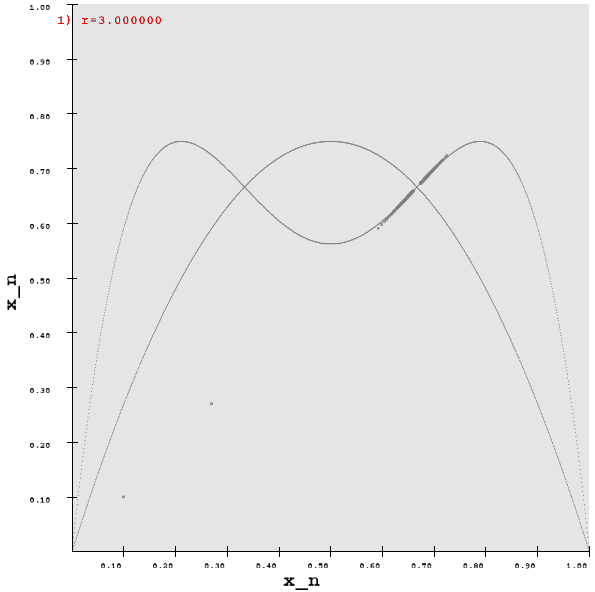
\includegraphics[scale=0.3]{r3}
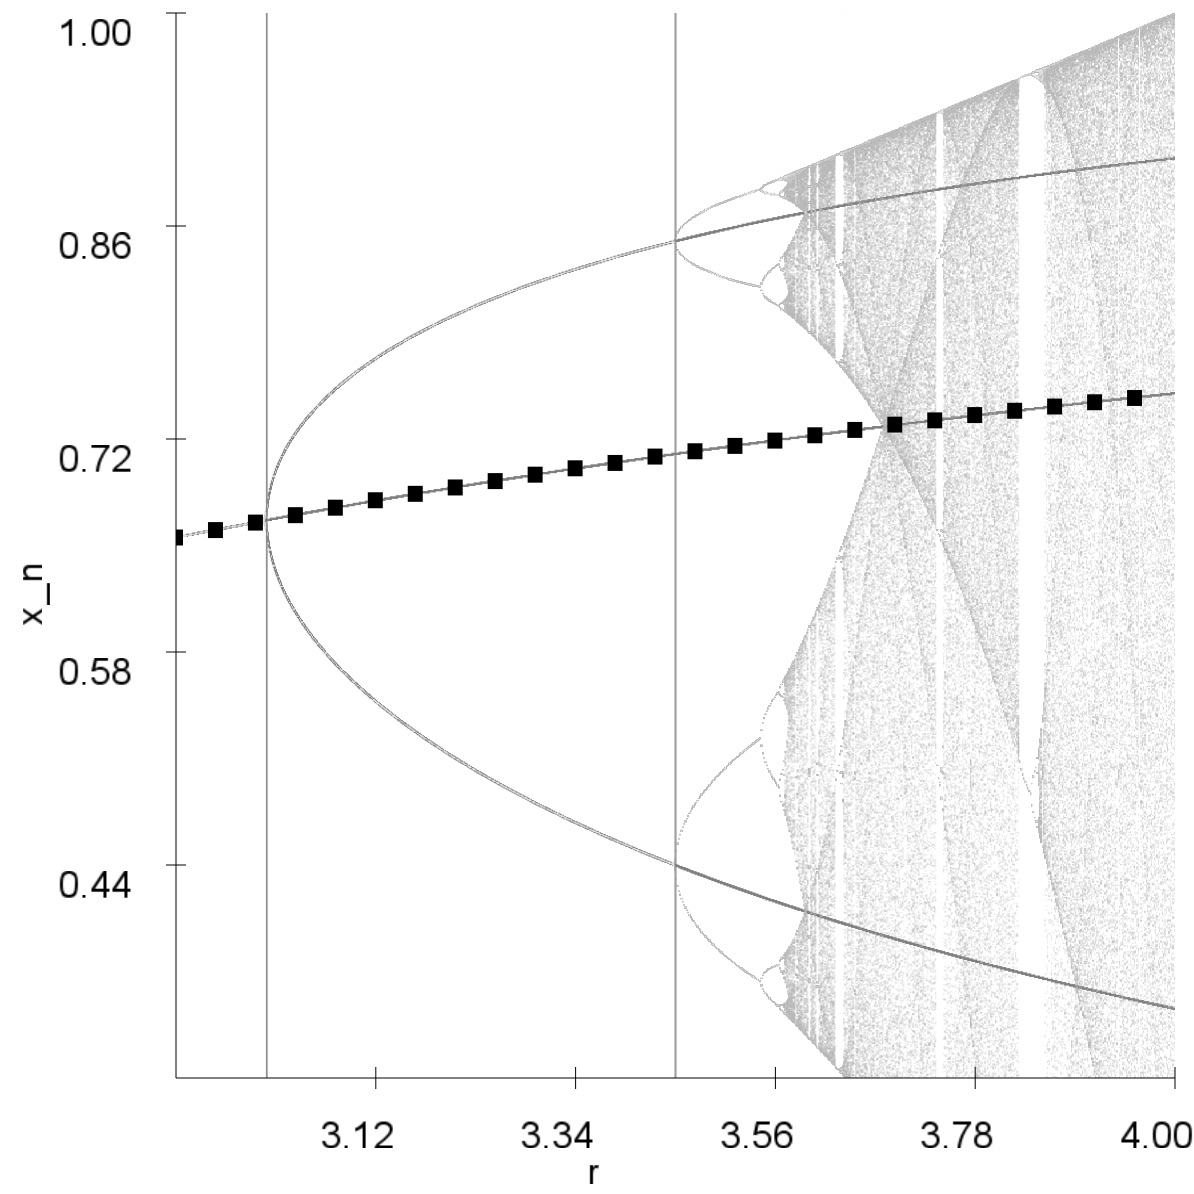
\includegraphics[scale=0.3]{analy-periodenv}
\newline
\subsection{ Stabilitätsbedingung }
Ein Fixpunkt ist stabil, wenn gilt:
$$\mid f'(x)\mid <1$$
Im Fall der logistischen Abbildung gilt
$$\frac{d}{dx}f(x)=r-2rx=r(1-2x)$$
$$\frac{d}{dx}f^2(x)=-r^2(2x-1)(2r(x-1)x+1)$$
\newline
Es gilt zu lösen, für welche $r$ bei bekannten Fixpunkte die Stabilitätsbedingung erfüllt ist.
\newline
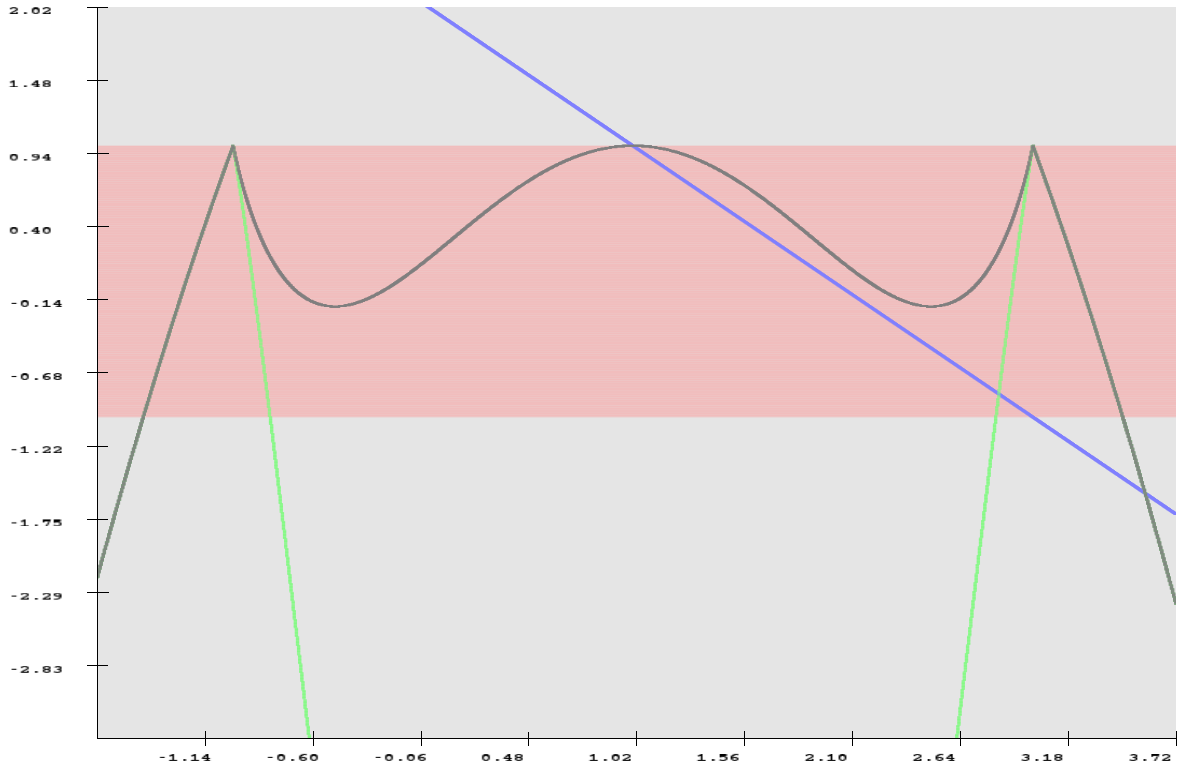
\includegraphics[scale=0.4]{stable_fixpoints}
\newline
Grafisch lässt sich ablesen, dass der Fixpunkt $x_3=\frac{\sqrt{r^2-2 r-3}+r+1}{2 r}$ (grüner Graph) für folgende Bereiche stabil ist:
$$-1.45<r<-0.82 \Rightarrow -1.45 < r \leq -1$$
$$2.82<r<3.45 \Rightarrow 3 \geq r > 3.45$$
Der Fixpunkt $x_4=\frac{-\sqrt{r^2-2 r-3}+r+1}{2 r}$ (grauer Graph) ist im gesamten Bereich $-1.45<r<3.45$ stabil aber da der Fixpunkt ebenfalls nur für $r \leq -1 \land r \geq 3$ existiert gilt der selbe Bereich wie für $x_3$. Die Fixpunkt sind dort stabil, wo sich der graue und der grüne Graph in der Abbildung überlagern.
\section { Bifurctationsdiagramm}
\subsection { Logistische Abbildung }
asdf
\subsection { Sinus Abbildung }
asdf
\section{ Feigenbaumkonstante}
\subsection {Lyapunov}
Eine Möglichkeit die Feigenbaumkonstante zu berechnen ist über die Nullstellen des Lyapunov-Exponenten. Gerade an diesen Stellen kommt es zu einer Periodenverdopplung. Dann lässt sich die Feigenbaumkonstante durch
$$\delta = \lim_{n \rightarrow \infty}\frac{a_{n-1}-a_{n-2}}{a_n-a_{n-1}}$$
, wobei die $a_n$ der Parameter ist bei dem die n-te Periodenverdopplung auftritt.
\newline
Für dern Lyapunov-Exponenten gilt:
$$\lambda(x_0) = \lim_{N \rightarrow \infty}\lim_{\epsilon \rightarrow 0} \frac{1}{N}\log{\mid \frac{f^N(x_0+\epsilon)- f^N(x_0)}{\epsilon} \mid} $$
oder auch
$$\lambda(x_0) = \lim_{N \rightarrow \infty} \frac{1}{N} \sum_{i=0}^{N-1}  \log{f'(x)} $$
Zweite Formel implementiert als OpenGL Kernel für die logistische Abbildung:
\begin{lstlisting}
float g(float r, float x) {
    return r * x * (1-x);
}
vec4 f(vec4 x) {
    float x0 = 0.4;
    float eps = 0.0001;
    float n = 10000;
    float summe = x0;
    for (int i = 1; i <= n - 1; i+=1) {
        x0 = g(x.x, x0);
        summe += log(abs(g(x.x, x0+eps)-g(x.x, x0))/eps);
    }
    return vec4(x.x, summe/n, 0, 0.5);
}
\end{lstlisting}
\begin{figure}
	\centering
	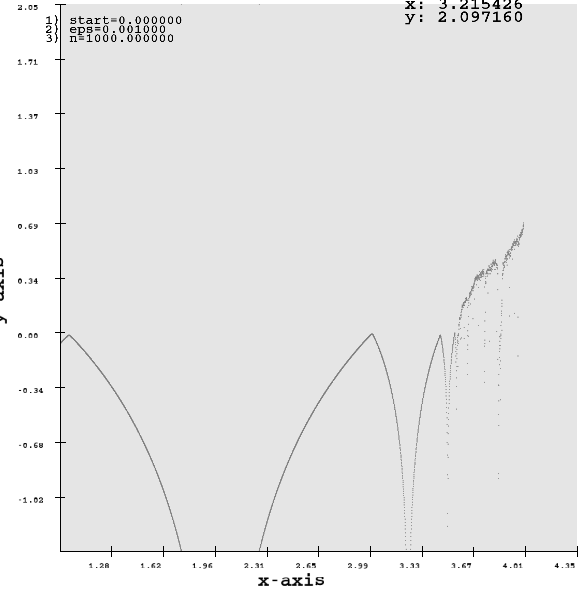
\includegraphics[scale=0.65]{lyapunov_1000}
	\caption{Lyapunov mit N=1000 und $\epsilon=0.001$ (Logistische Abbildung). Parameter r auf der x-achse und $\lambda(x_0)$ auf y-achse, mit startwert $x_0=0.4$}
	\label{img:lyapunov_100}
\end{figure}
Wie erwartet ist eine Nullstelle bei $x=3$. Gucken wir uns allerdings den Bereich für $x=3$ genauer an, so stellen wir eine gewisse Ungenauigkeit fest (vgl. nächste Abbildung). Da wir für die Feigenbaumkonstante möglichst genau die Stellen an denen Periodenverdopplung auftritt identifizieren wollen, müssen wir die Parameter entsprechend modifizieren. Die Fluktuation nehmen zu, wenn $\epsilon$ kleiner wird.
\begin{figure}
	\centering
	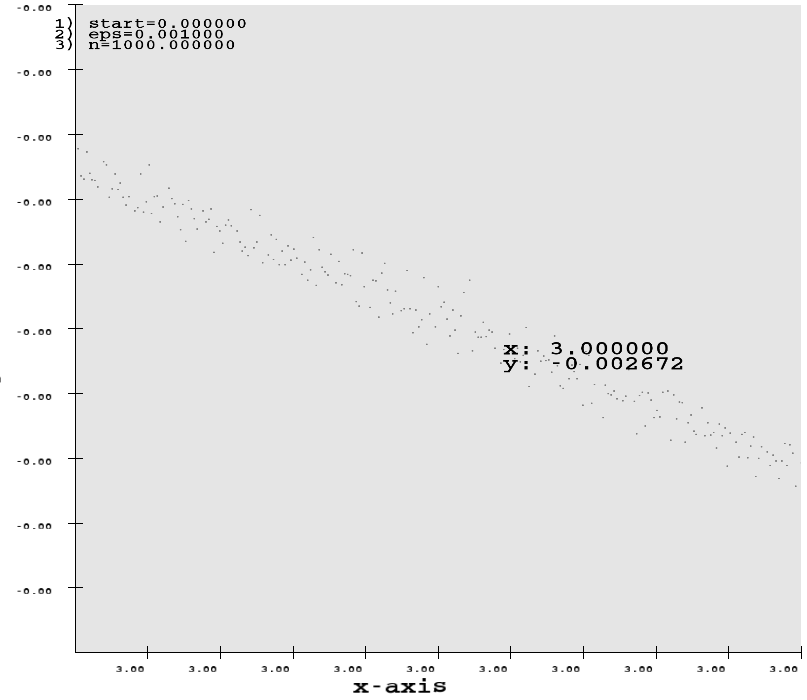
\includegraphics[scale=0.50]{lyapunov_1000_at_3}
	\caption{1. Bei $x=3$ erhalten wir einen von 0 verschiedenen Wert ($\lambda\approx-0,0027$) 2. Wie stellen fest das der Lyapunov-Exponent für unterschiedliche r fluktuiert.}
	\label{img:lyapunov_1000_at_3}
\end{figure}
\newline
@TODO: Bei N -> 13000 und epsilon < 0.00001 kommt man schon ganz gut dran!
1. Verhalten wenn man erst später anfängt zu summieren
2. Bei gegebener Konfiguration für r=3 messen mit Fehler etc.
3. Weitere Periodenverdopplungen grafisch identifizieren. (Domain hoch setzen für bessere Genauigkeit)
4. Ursache für Fluktuationen?? Und Möglichkeit diese Fluktuationen zu mitteln!?
5. Mit gemittelter Fluktuation in OpenCL nicht-grafisch Nullstellen identifiezieren (double precision!!! -> Fehler der durch float64 berücksichtigt werden muss)

\section { Duffing-Gleichung}
Wir betrachten nun ein angetrieben und gedämpften Oszillator. Als Unterschied zum klassischen Harmonischen Oszillator wird der Term mit der Federkonstante kubisch.
$$\ddot{x}+\lambda\dot{x}+\beta x^3=\epsilon\cos{\Omega t}$$
Diese DGL lässt sich nun nicht mehr analytisch berechnen.
Im Folgenden lösen wir die Gleichung mit der Euler-Methode als auch mit dem Runge-Kutta Verfahren.
$$\frac{dy}{dt}=\epsilon\cos{\theta}-\lambda y - \beta x^3$$
$$\frac{dx}{dt}=y$$
$$\frac{d\theta}{dt}=\Omega$$
\subsection { Attraktoren }
Parameter:
$$\epsilon = 0,2, \lambda = 0,08, \beta = 1, \Omega = 1$$
- Unterschiede Runge Kutta Euler (unterschiedliche attraktoren)
\newline
- stabile / instabile Trajektorien --> parameter $h = \frac{Zeit}{Iterationen}$
\newline
- Optimierung durch Schrittweiten adaptierung
\newline
- lyapunov??
\subsection{ Poincareschnitt }
Stichwort: Seltsame Attraktoren, Hasudorff-Dimension, Fraktale

\section {LDR-Oszillator}


\section{ Literatur }
\begin{itemize} 
\item Nichtlineare Dynamik und Chaos - Physikalisches Praktikum für Fortgeschrittene Universität Hamburg
\end{itemize}




\end{document}







